%!TEX root = ../main.tex
\section{Modelling a DC motor}
This section deals with the modelling and parameterisation of a brushed DC motor, specifically the Pittmann 9234 24V servomotor.
Figure \ref{fig:dcmotormodel} is a simple model of a DC motor.
The parameters of this model will be estimated by experimentation.

\begin{figure}[!h]
	\centering
	\includegraphics[width=\linewidth]{graphics/dcmotormodel.png}
	\caption{Simulink model of a brushed DC motor.}
	\label{fig:dcmotormodel}
\end{figure}


\subsection{Armature Resistance - $R_a$}
The armature resistance, $R_a$ in figure \ref{fig:dcmotormodel}, can be found simply by applying Ohm's law.
The current through a resistor is well defined when a voltage is applied across it.

\begin{figure}[!h]
	\centering
	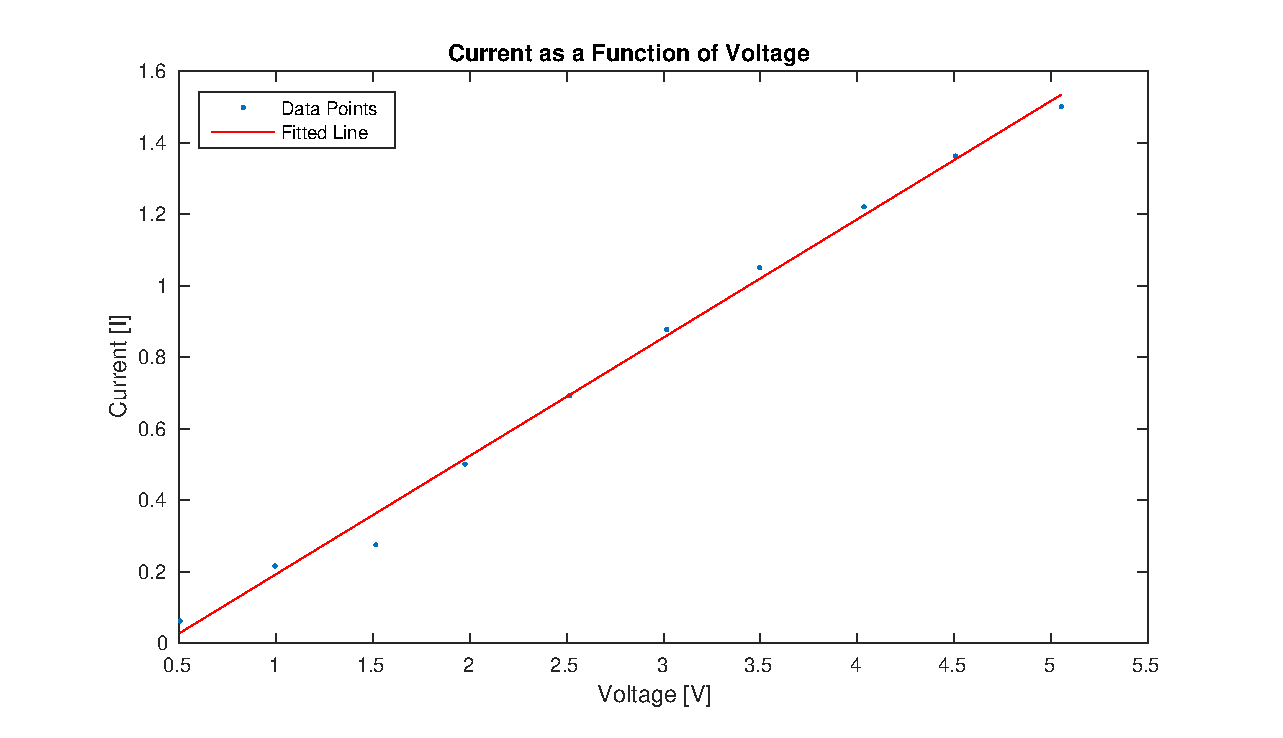
\includegraphics[width=\linewidth]{graphics/raplot}
	\caption{Current as a function of voltage with the rotor blocked.}
	\label{fig:raplot}
\end{figure}

However, when the rotor is spinning, the circuit produces back-EMF.
This counters the input voltage, effectively lowering the current through $R_a$.
In order to avoid this effect the rotor is blocked.
Since, with a blocked rotor, there will be no change in voltage in the system, the inductor acts as a short circuit, reducing the circuit to a voltage across a resistor. 

Figure \ref{fig:raplot} shows the data collected in order to determine the value of the armature resistance.
A voltage is applied across the terminals at 0.5 V.
According to the datasheet \cite{pittmann} the current at maximum allowed continuous torque is 1.75 A.
This current is reached at 5 V, therefore, the measurements stop there.
As can be seen from the figure, a line is fitted to the data.
This is done using the linear least squares method with the following result:
$$I(V)=0.331\cdot V-0.138$$
with $R^2=0.994$.
Since for the plot $I(V)$:
$$R_a = \frac{1}{\text{slope}} = 3.02\Omega$$
However, at $I(0)$ the model will result in a small negative current.
This is obviously not correct; no current would be expected at zero voltage.
Adjusting the model such that it will intersect the origin results in a higher resistance of $R_a=3.43\Omega$.

\subsection{Motor inductance - $L_a$}
The inductance of the motor, $L_a$ in figure \ref{fig:dcmotormodel}, can be found by looking at the transient response of the motor. 
When the motor is stalled there is no back-EMF in the circuit. The motor can then be modelled as a simple RL-circuit. 
An RL-circuit has a known time constant $\tau$.
$$\tau = \frac{L}{R_{total}}$$
The time onstant is defined as the time it takes for the voltage across the component to rise or fall to $\frac{1}{e}$ of the final value.
Measuring the time constant would require measuring the voltage across the inductor or the resistor in the motor. This is not possible as these are built-in. 
Therefore an extra resistor, $R_e$, was put in series with the motor and the voltage across it was measured by an oscilloscope. 
$$\tau = \frac{L}{R_{total}} = \frac{L_a}{R_a+R_e}$$
Rearraring the formula for $\tau$ yields an expression for $L_a$: 
$$L_a = \tau * (R_a + R_e)$$
To give the circuit a step signal it was given a voltage of 8 V by a power supply and then the terminals of the power supply was  short circuited by connecting the terminals with a wire. Thus giving it a step signal with a initial value of 8 V and a final value of 0 V.
The experiment was repeated 10 times. $\tau$ can be found by locating the time where the measured voltage is equal to $\frac{1}{e}$ of the initial voltage.

\subsubsection{Experiment}
The extra resistor, $R_e$, was measured by a multimeter to have a value of $32.97\Omega$.
Then the circuit was given the step signal while measuring the voltage.
The transient responses measured across $R_e$ can be seen in figure \ref{fig:trans_plot}.

\begin{figure}[!h]
	\centering
	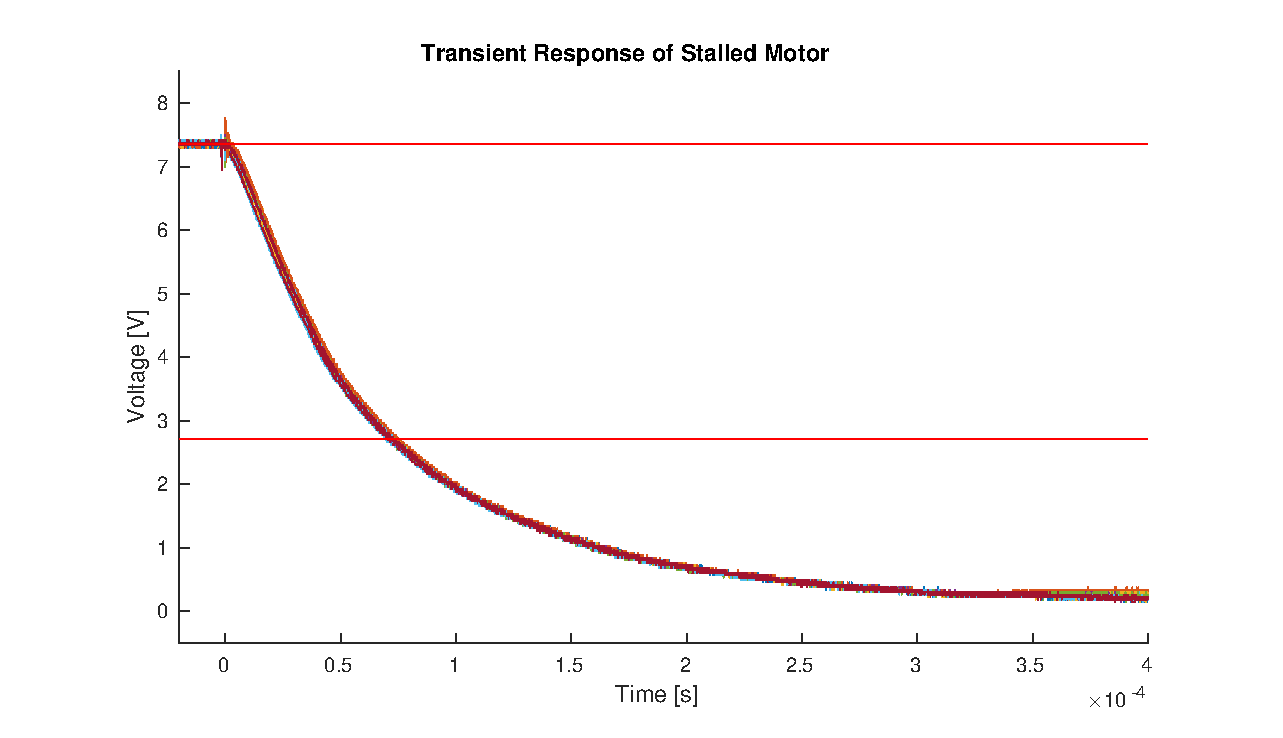
\includegraphics[width=\linewidth]{graphics/transient_32ohm}
	\caption{Transient responses measured across $R_e$. The red vertical lines represent the initial voltage, $V_0$, and $\frac{1}{e} \cdot V_0$.}
	\label{fig:trans_plot}
\end{figure}


$\tau$ was found to be 0.713 $\cdot 10^4 s$, by taking the average of the found values from the 10 experiments.
The average value of $L_a$ was then found to be 2.6 mH. The value is only $3.83\%$ higher than the value in the datasheet.

\subsubsection{Discussion}
Only the voltage across $R_e$ is measured, which is problematic as it is assumed in the formula that the transient response is measured across the whole resistance of the circuit. Choosing a value for $R_e$ that is much larger than $R_a$ would minimize the problem.
The experiment was done with values of $R_e$ ranging from $33\Omega$ to $3.3K\Omega$.
Results generally showed that higher values of $R_e$ yielded more difference between the calculated values of $L_a$ and the value given in the datasheet.